\begin{figure}[H]
\centering
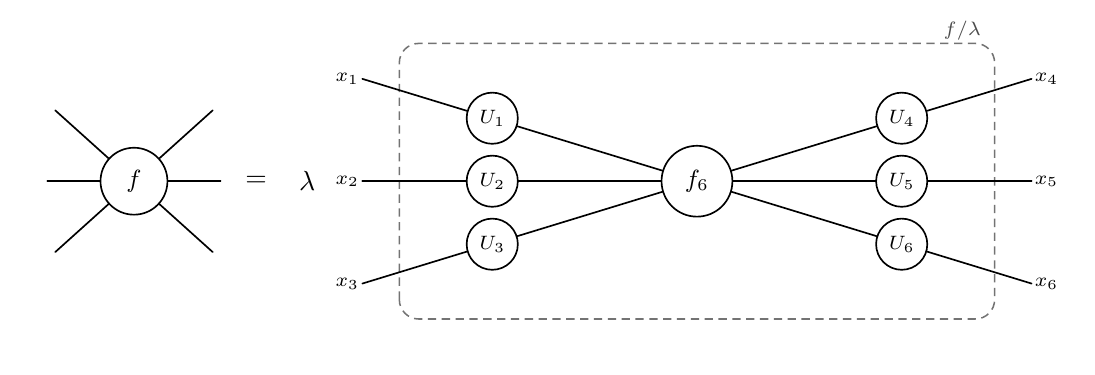
\begin{tikzpicture}[
    wire/.style={draw=black, line width=0.6pt, line cap=round},
    boundary/.style={draw=black!55, densely dashed, line width=0.55pt,
        rounded corners=7pt},
    signature/.style={draw=black, circle, fill=white, minimum size=7.2mm,
        inner sep=0pt, line width=0.6pt, font=\small},
    local unitary/.style={signature, minimum size=6.5mm, font=\scriptsize},
    port label/.style={font=\scriptsize, inner sep=1pt}
]
    \path[use as bounding box] (0,0) rectangle (13.2,4.05);

    % The six-ary signature f.
    \coordinate (f) at (1.35,2.10);
    \draw[wire] (0.35,3.00) -- (f);
    \draw[wire] (0.25,2.10) -- (f);
    \draw[wire] (0.35,1.20) -- (f);
    \draw[wire] (f) -- (2.35,3.00);
    \draw[wire] (f) -- (2.45,2.10);
    \draw[wire] (f) -- (2.35,1.20);
    \node[signature, minimum size=8.5mm] at (f) {$f$};

    \node[font=\normalsize] at (2.90,2.10) {$=$};
    \node[font=\normalsize] at (3.55,2.10) {$\lambda$};

    % The gadget for (U_1 \otimes \cdots \otimes U_6)f_6.
    \draw[boundary] (4.72,0.35) rectangle (12.28,3.85);
    \node[port label, anchor=south east, text=black!70]
        at (12.15,3.85) {$f/\lambda$};

    \coordinate (f6) at (8.50,2.10);
    \draw[wire] (4.25,3.40) -- (f6);
    \draw[wire] (4.25,2.10) -- (f6);
    \draw[wire] (4.25,0.80) -- (f6);
    \draw[wire] (f6) -- (12.75,3.40);
    \draw[wire] (f6) -- (12.75,2.10);
    \draw[wire] (f6) -- (12.75,0.80);

    \node[local unitary] at (5.90,2.90) {$U_1$};
    \node[local unitary] at (5.90,2.10) {$U_2$};
    \node[local unitary] at (5.90,1.30) {$U_3$};
    \node[local unitary] at (11.10,2.90) {$U_4$};
    \node[local unitary] at (11.10,2.10) {$U_5$};
    \node[local unitary] at (11.10,1.30) {$U_6$};
    \node[signature, minimum size=9mm] at (f6) {$f_6$};

    \node[port label, left]  at (4.25,3.40) {$x_1$};
    \node[port label, left]  at (4.25,2.10) {$x_2$};
    \node[port label, left]  at (4.25,0.80) {$x_3$};
    \node[port label, right] at (12.75,3.40) {$x_4$};
    \node[port label, right] at (12.75,2.10) {$x_5$};
    \node[port label, right] at (12.75,0.80) {$x_6$};
\end{tikzpicture}
\caption{Gadget form of~\eqref{eq:f6-local-unitary-form}.
The dashed enclosure realizes
$(U_1\otimes\cdots\otimes U_6)f_6=f/\lambda$, where $U_i$ is an binary extension on variable $x_i$ of $f_6$.
This need not be an $\mathcal F$-gate, since the local unitaries $U_i$ maybe can not be realized in $\mathcal F$.}
\label{fig:f6-local-unitary-gadget}
\end{figure}
